\section{Application existante}

\subsection{Présentation de l'application}
L'application sur laquelle nous travaillons est écrite en C++ avec l'utilisation de QtCreator. Le 
programme a été développé par l'équipe Fox et par des étudiants. Cette application il a fait 
l'objet de divers améliorations auparavant.\\

\subsection{Architecture}
L'application fournis est orientée objet, celle-ci est découpé en Business Objects\footnote{les objets 
métier s'occuppent d'une tâche précise}. Ces Business Objects sont hiérarchisé dans une pyramide, les 
objets métiers en haut de cette pyramide sont les plus abstrés et utilise les resultats de l'étages infèrieur. 
Les objets métiers en bas de la pyramide sont les plus proche du flux vidéo brut.

%TODO explications des couche

\begin{figure}[H]
  \centering
  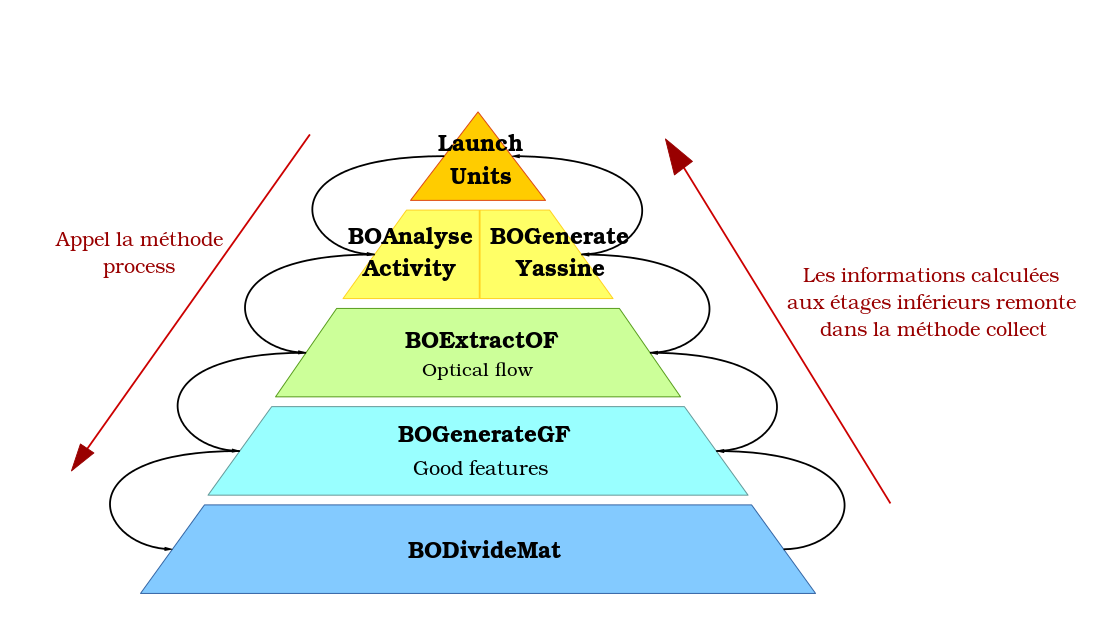
\includegraphics[width=12cm]{image/pyramide.png}
  \caption{Processus d'extraction des informations pyramidal sur le flux vidéo}
\end{figure}

%TODO explications de notre couche

\subsection{Reconnaissance du visage : Viola et Jones}
L'application est divisée en deux parties. La première recherche le visage grâce à
l'algorithme de Viola et Jones et la seconde recherche les yeux dans la région délimitée
précédemment.\\

L'algorithme de Viola et Jones\cite{Viola04robustreal-time} est une méthode qui a été créée pour la reconnaissance de visage dans une 
image. Cette méthode s'est par la suite généralisée à toutes sortes d'objets. L'algorithme nécessite une 
base de connaissances composée des caractèristiques de l'objet recherché. Cette base de connaissances est utilisé dans un 
apprentissage supervisé, c'est à dire que l'algorithme a besoin de données représentant
l'objet à détecter pour classifier les caractèristiques de celui-ci.\\

Cette algorithme est basé sur des caractèristiques pseudo-Haar qui crée des masques rectangulaires et adjacentes
dans différente zone de l'image. Chaque masque calcule l'intensité des pixels qu'il contient, puis l'algorithme fait
la différence entre les masque blanc et les masque noir. Cette méthode va permettre de détecter des contours ou des changements de 
texture.\\

\begin{figure}[H]
\center

\includegraphics[width=5cm]{image/pseudo_haar.png}
\caption{Exemple de caractèristiques pseudo-Haar utilisé pour l'algorithme Viola et Jones}
\end{figure}

Pour améliorer les perfomance de leur algorithme, Viola et Jones utilise la méthode Adaboost. Son
principe est de séléctionner les caractèristiques les plus performante pour la détection de l'objet grâce à
un calcule de probabilité utilisant l'entropie\footnote{valeur mesurant l'incertitude d'une données} des données.

\subsection{Suivi des yeux}
%TODO voir quel algo est utilisé à la base -> gaetan?

